

\documentclass{article}
\usepackage{graphicx}
\usepackage{hyperref}


\title{Sprint 3.5-4 Prototypes}
\date{4/9/2016}

\begin{document}
	\maketitle
	\newpage
	
	\section{Introduction}
	This is a prototype report to give the status of the UAV Lander project after sprints 3.5 and 4. The team was able to make progress and achieve the goals of manual flight and autonymous GPS waypoint navigation.
	
	\section{Manual Flight}
	After the UAV was successfully assembled, the team needed to do more than just spin the motors in the robotics lab. The UAV was taken up to the school gym, where the team was able to sucessfully fly it under manual control, sending commands directly over radio to the flight controller.
	
	\begin{figure}[h]
		\centering
		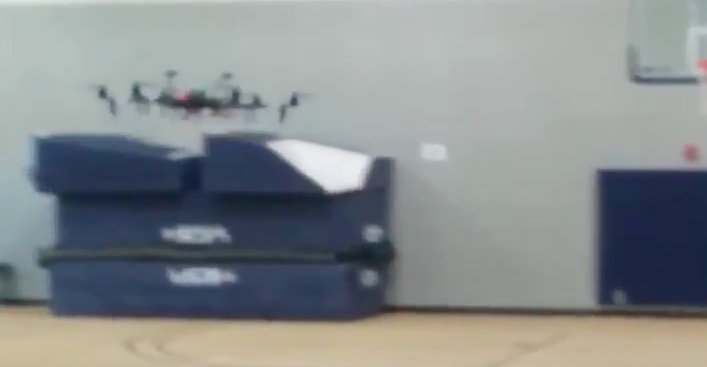
\includegraphics[width=0.5\textwidth]{gym.png}
		\caption{UAV Flying in the Gym}
	\end{figure}
	
	The manual flight in the gym was a good measure of first success for the team, as it showed that the UAV was assembled properly, and that the flight controller functioned well with our hexacopter setup. One thing that was mentioned to us here was that the handheld radio that the team was using was designed for fixed-wing aircraft such as model airplanes. This posed a problem when flying the UAV under manual control, because the throttle inputs would click into place, rather than being continuous. This was a problem because in order to maintain altitude, the pilot would have to constantly be clicking the throttle stick between various positions.
	
	\section{Autonymous GPS Waypoint Navigation}
	Shortly after the indoor manual flight, the team was able to get the UAV set up for autonymous GPS waypoint navigation. This is important to the project because one of the major tasks is to build a UAV that is able to navigate through a set of GPS waypoints. The results of the team's testing of the waypoint navigation point to the possibility that GPS will be sufficient to allow the UAV to position itself over the landing pad. This means that little to no work should need to be put into developing a search algorithm to get the UAV to locate the pad after flying to the waypoint, in the event that GPS was inaccurate.
	
		\begin{figure}[h]
			\centering
			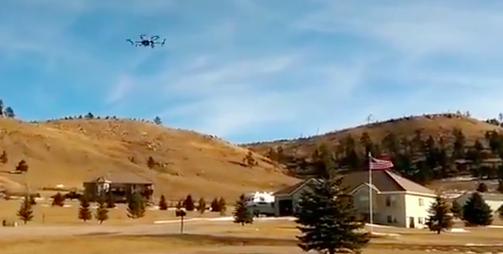
\includegraphics[width=0.5\textwidth]{wind.png}
			\caption{UAV Navigating Through Waypoints in the Wind}
		\end{figure}
		
	One exciting result during testing was that the team flew the UAV on a windy day. In the above image, you can see that a flag is blowing in the wind. The UAV did not show any signs of being blown around, even despite this.

		\begin{figure}[h]
			\centering
			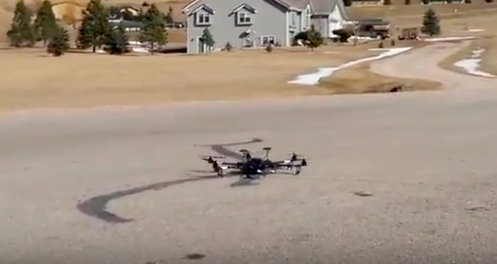
\includegraphics[width=0.5\textwidth]{start.png}
			\caption{Location of UAV Before Takeoff}
		\end{figure}	

		\begin{figure}[h]
			\centering
			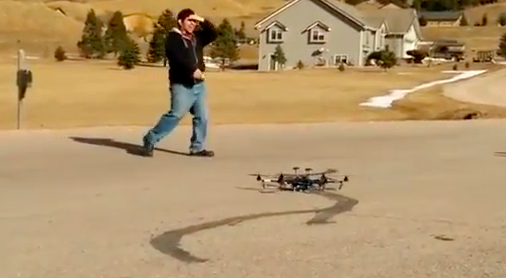
\includegraphics[width=0.5\textwidth]{end.png}
			\caption{Location of UAV After Landing}
		\end{figure}	

	The above two images show just how accurate the GPS waypoint navigation was. The UAV started at the location in the first image, took off, flew through a series of waypoints, and landed at the location in the second image. This test was done the same day, so this result was observed even in the wind. Another success that makes the team believe that GPS is reliable is that during these tests, one of the motor arms on the UAV had come loose and rotated. The flight controller was still able to keep the UAV under control, even despite these problems
	
	
\end{document}